\documentclass[aspectratio=169]{beamer}
\usepackage{amsmath}
\usepackage{amssymb}
\usepackage{amsfonts}
\usepackage{graphicx}
\usepackage{luatexja} 
\usepackage{comment}
\usepackage{bm}
\usepackage{setspace}
\usepackage{caption}
\usepackage{hyperref}
\usepackage{natbib}
\bibliographystyle{unsrt}

\usetheme{LightTheme}
\setbeamertemplate{footline}[frame number]
\setbeamertemplate{navigation symbols}{}
\setlength{\baselineskip}{10pt}
\begin{document}

% タイトルフレーム
\title{\Large 木幅アルゴリズムの学習システムの構築}
\subtitle{進捗状況} 
\author{\small B4 小林紹子} % 必要に応じて変更・削除
\date{\small\today} % 必要に応じて変更・削除

\begin{frame}
    \titlepage
\end{frame}

\begin{frame}{目次}
    \tableofcontents
\end{frame}

\section{学習システム構築の目的}

\begin{frame}{研究背景}
    \begin{itemize}
        \setlength{\parskip}{1.5em}
        \item 木幅はグラフ構造理論などアルゴリズム設計で重要な概念.
        \item しかし,
        \begin{itemize}
            \setlength{\parskip}{1em}
            \item 理解が難しい(抽象的な概念,木分解の構築の難しさ)
            \item 日本語で学べる教材や可視化・インタラクティブな教材が少ない.
        \end{itemize}
        \item \Rightarrow 「木幅アルゴリズムを直感的に学べる教材」が求められている.
    \end{itemize}
\end{frame}

\begin{frame}{研究目的}
    \begin{itemize}
        \setlength{\parskip}{1.5em}
        \item 木幅や木分解の理解を支援する学習サイトを開発する.
        \item 対象:アルゴリズムをある程度学習している人(例:情報系学生).
        \item 目的:
        \begin{itemize}
            \setlength{\parskip}{1.5em}
            \item 定義の理解促進.
            \item アルゴリズムの可視化による直感的理解.
        \end{itemize}
    \end{itemize}
\end{frame}

\section{要件定義}

\begin{frame}[allowframebreaks]{要件定義}
    \begin{enumerate}
        \setlength{\parskip}{1em}
        \item 問題管理機能(サーバー側)
        \begin{itemize}
            \item 問題文,画像,正答を含む問題データを保持.
            \item API経由でデータのやり取りを行う.
        \end{itemize}
        \item 問題表示機能(クライアント側)
        \begin{itemize}
            \item サーバーから問題リストを取得して表示.
            \item 問題文と対応する画像の表示.
            \item ユーザーが解答を選択・入力可能.
        \end{itemize}
        \newpage
        \item 解答送信・結果表示機能
        \begin{itemize}
            \item 解答送信時にサーバーにリクエストを送信.
            \item サーバー側で判定し,結果を返す.
            \item ページ遷移せずに喧嘩を即時表示.
        \end{itemize}
        \item インタラクティブに図をマウス等で操作.
        \begin{itemize}
            \item 操作し変更された図の頂点をデータとして保持.
            \item 解答として送信可能.
        \end{itemize}
        \item 相手の解答パターンに合わせた正解を自動生成.
        \begin{itemize}
            \item それ以前に選択された答えによって異なる解答が得られる.
            \item サーバー側でインタラクティブに生成.
        \end{itemize}
    \end{enumerate}
\end{frame}

\begin{frame}{将来的な拡張要件}
    \begin{itemize}
        \setlength{\parskip}{1.5em}
        \item 管理者画面での問題追加・削除.
        \item ユーザー登録.
        \item 回答履歴・正答率の記録.
    \end{itemize}
\end{frame}

\section{Webアプリケーション}

\begin{frame}{このまま説明する前に}
    \begin{itemize}
        \setlength{\parskip}{1.5em}
        \item これから使用技術について説明したい.
        \item 事前に説明してみたら,井口先生にウェブプログラミングを履修していない学生が多いと言われた.
        \item 今後のためにもまずは基本的なWebアプリケーションについての仕組みを説明します...
    \end{itemize}
\end{frame}

\subsection{基本的なWebサイトの構成}
\begin{frame}{クライアントとサーバー}
    \begin{itemize}
        \setlength{\parskip}{1.5em}
        \item \textbf{クライアント}:サーバーに指示を出すデバイス(例:PC, スマートフォン)\cite{server-client}.
        \item \textbf{サーバー}:\\サービスや機能を提供するコンピュータ.クライアントから要求された形に情報を加工したり,保存したりする役割がある.
                                サーバーにも役割によって種類がある.\\
        \vspace{1em}                                
        \begin{itemize}
            \setlength{\parskip}{1em}
            \item Webサーバー:Web関連のサービスを提供しているコンピュータ.
            \item メールサーバー:メール関連のサービスを提供しているコンピュータ.
            \item DNSサーバー:URLをIPアドレスに変換するコンピュータ.
        \end{itemize}                                
      {\tiny [1]サーバーとは?クライアントとは?それぞれの違い\url{https://menter.jp/blog/server-and-client}}  
        
    \end{itemize}
\end{frame}

\begin{frame}{リクエストとレスポンス}
    \begin{itemize}
            \setlength{\parskip}{1.5em}
            \item Webサイトを閲覧する際にクライアントからサーバーに通信することを「\textbf{リクエスト}」と呼ぶ.
            \item サーバーがリクエストを受け, クライアントに返答することを「\textbf{レスポンス}」と呼ぶ.
    \end{itemize}
    \begin{figure}
        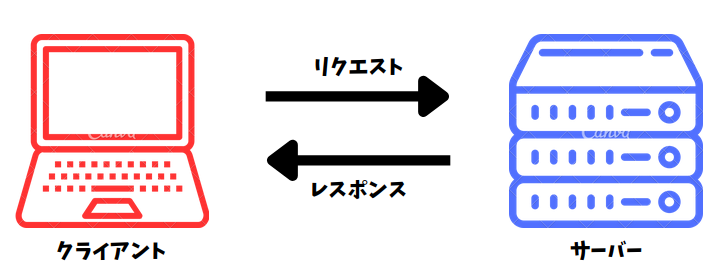
\includegraphics[scale=0.4]{server-and-client.png}
    \end{figure}
\end{frame}

\begin{frame}{WebアプリケーションとWebサイトの違い}
    \begin{itemize}
        \setlength{\parskip}{1.5em}
        \item \textbf{Webサイト}:常に同じHTMLをクライアントに返す.
        \item \textbf{Webアプリケーション}:\\表示内容をクライアントごとに動的に変化するHTMLを返す.
        \begin{enumerate}
            \setlength{\parskip}{1em}
            \item WebブラウザからURLを入力してEnter.\\リクエスト情報がWebアプリに送信(リクエスト).
            \item リクエストがWebアプリに届くと,リソース(HTML, CSS)をデータベースと連携して取得.
            \item ブラウザに返す(レスポンス).
        \end{enumerate}
    \end{itemize}
\end{frame}
\subsection{データベース}
\begin{frame}{データベース}
    \begin{itemize}
        \setlength{\parskip}{1.5em}
        
        \begin{columns}
        \begin{column}{0.55\textwidth}
        \item \textbf{データベース}:\\            
        \begin{itemize}
            \setlength{\parskip}{1em}
            \item 構造化した情報,データの組織的な集合\cite{database}.
            \item 通常はコンピュータ・システムに電子的に格納.
            \item \textbf{データベース管理システム(DBMS)}で制御.
        \end{itemize}
        \end{column}            
        \begin{column}{0.3\textwidth}
            \begin{figure}
                
\includegraphics[scale=0.2]{database.png}
            \end{figure}
        \end{column}
        \end{columns}
        \item \textbf{データベース管理システム(Database Management System)}:\\
        \begin{itemize}
            \setlength{\parskip}{1em}
            \item データベースとそのエンドユーザー・プログラムの間でインタフェースとして機能.
            \item データベースの監視・制御を容易にする.
            \item 例)MySQL
        \end{itemize}
    \end{itemize}
    {\tiny \cite{database}データベースとは\url{www.oracle.com/jp/database/what-is-database/}}  
\end{frame}

\begin{frame}{Webアプリケーションの流れ}
    \begin{figure}
        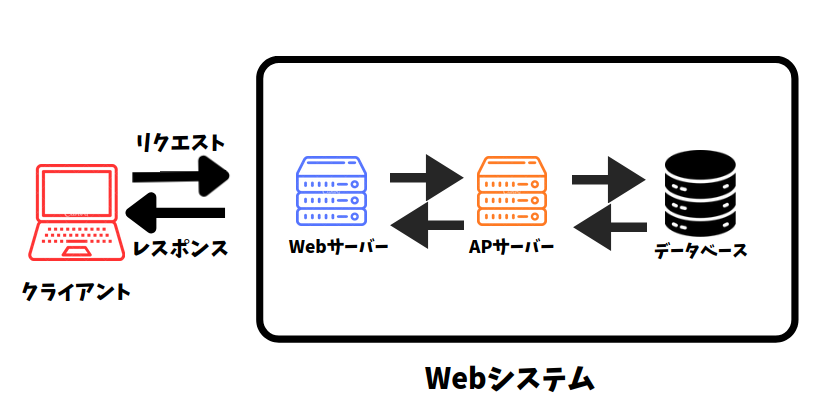
\includegraphics[scale=0.4]{websystem.png}
    \end{figure}
\end{frame}

\begin{frame}{WebサーバーとAPサーバー}
    \begin{itemize}
        \setlength{\parskip}{1.5em}
        \item \textbf{Webサーバー}:\\
        \begin{itemize}
            \setlength{\parskip}{1em}
            \item HTTPリクエストを受け取る\cite{webserver}.
            \item HTMLやCSS,画像などでレスポンスを返す.
        \end{itemize}
        \item \textbf{APサーバー(Webアプリケーションサーバー)}:\\
        \begin{itemize}
            \setlength{\parskip}{1em}
            \item Webサーバから受け取った情報を処理\cite{apserver}.
            \item 必要に応じてデータベースサーバにアクセス.
            \item 動的コンテンツの生成・管理.
        \end{itemize}
    \end{itemize}
    \textbf{Webサーバはユーザーとの窓口.\\APサーバはユーザーのリクエストに応じた対応をおこなうバックヤード.}
\end{frame}
\subsection{Webアプリケーションの流れ}
\begin{frame}[allowframebreaks]{Webサイトがブラウザに表示されるまでの大まかな流れ}
    \begin{enumerate}
        \setlength{\parskip}{1em}
        \item Webサーバーにアクセスしてリクエストを送信.
        \item Webサーバーがリクエストを受け取り,解析.
        \item APサーバーが処理を実行.(DB問い合わせなど)
        \begin{figure}
            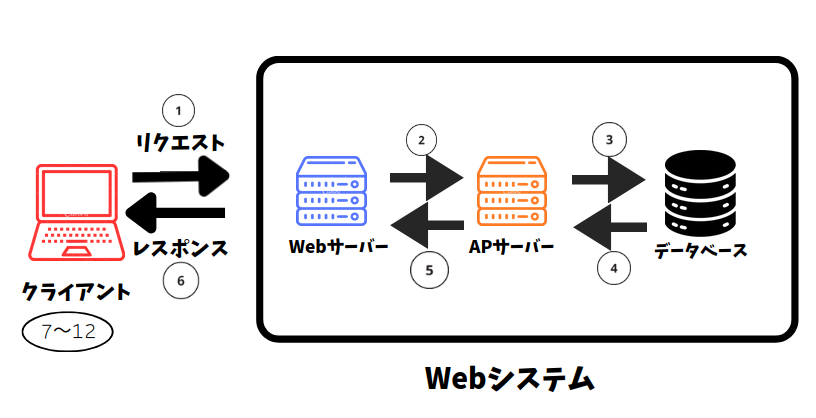
\includegraphics[scale=0.25]{webfloat.png}
        \end{figure}
        \newpage
        \item DBから情報を取得.
        
        \item 静的なHTMLとJavascriptコード or JSONなどのデータをWebサーバーに返す.
        \item Webサーバーがレスポンスとしてクライアントに送信.
        \begin{figure}
            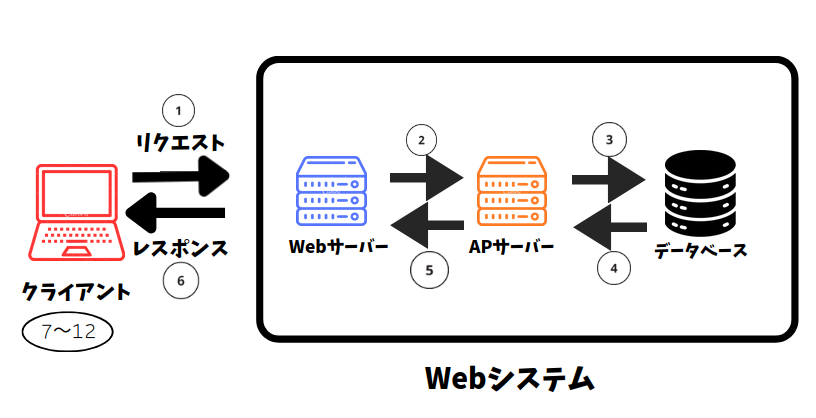
\includegraphics[scale=0.25]{webfloat.png}
        \end{figure}
        \newpage
        \item ブラウザ(クライアント)がHTMLを解析.DOMツリーを構築.

        \item CSSを読み込み,解析.CSSOMツリーを構築.
        
        \item Javascriptを読み込み実行.動的な処理(データ取得・DOM操作など)を行う.
        \begin{figure}
            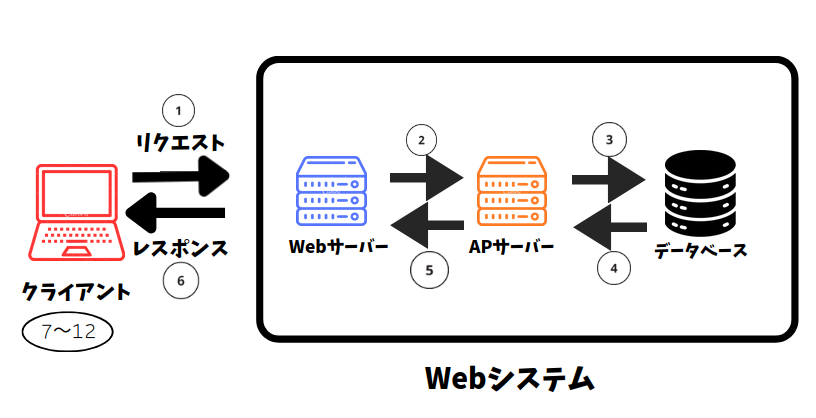
\includegraphics[scale=0.25]{webfloat.png}
        \end{figure}
        \newpage
        \item DOMツリーとCSSOMツリーを合成してレンダーツリーを構築.
        \item レイアウト計算・ペイント.
        \item 画面にレンダリング.
        \begin{figure}
            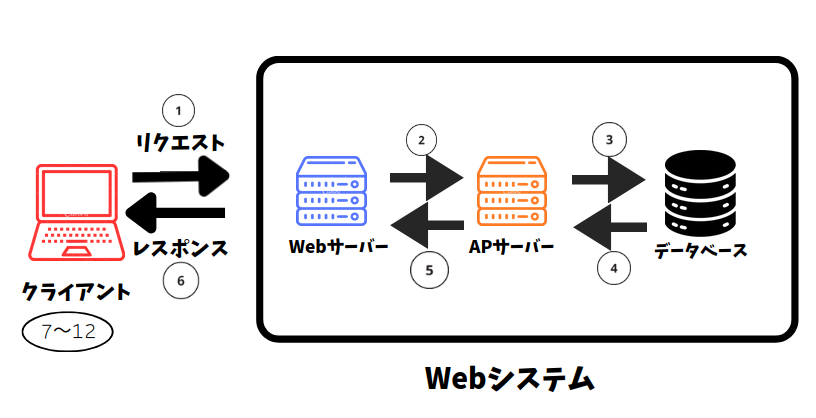
\includegraphics[scale=0.25]{webfloat.png}
        \end{figure}
    \end{enumerate}
    
\end{frame}
\section{サーバーが返すHTMLについて}
\subsection{SSR(Server Side Rendring)}

\begin{frame}{SSR(Server Side Rendring)}
    サーバーが返すHTMLにもどの程度の完成度にするか違いがある.\\
    \begin{itemize}
        \setlength{\parskip}{1em}
        \item \textbf{SSR(Server Side Rendring)}
        \begin{itemize}
            \setlength{\parskip}{1em}
            \item 登場:2000年代前半~中盤.(PHP, Ruby on Railsなど)
            \item ユーザーがページを開く度にサーバーがHTMLを「最初から全部生成」して返す.
            \item クリックなどの遷移も毎回サーバーにリクエスト.
            \item ブラウザはHTMLを受け取ってDOMツリーを作る.
        \end{itemize}
        \item \textbf{特徴}
        \begin{itemize}
            \setlength{\parskip}{1em}
            \item 表示が遅い(ページ全体を毎回描きなおす).
            \item SEO(検索エンジン対策)には強い.
        \end{itemize}
    \end{itemize}
\end{frame}

\begin{frame}{React}
    \begin{itemize}
        \setlength{\parskip}{1em}
        \item 2011年Facebook社(現Meta社)のソフトエンジニアがReactの前進となるプロトタイプを開発.2013年にオープンソース化.
        \item 画面の見た目を管理するための仕組みをライブラリ化したもの.
        \item HTMLを直接書かず,「状態に応じてUIを自動で作る」仕組みを持つ.
        \item 特徴
        \begin{itemize}
            \setlength{\parskip}{1em}
            \item 宣言的View:あらかじめ変更される部分を{}で囲むなど変更されない部分と区別して設計.
            \item コンポーネントベース:部品を組み立てるように作成する.容易+再利用可能になる.
            \item 仮想DOM:実際のDOMを直接操作せず,メモリ上にツリー構造を作り,変化部分だけを検出して更新する.
        \end{itemize}
    \end{itemize}    
\end{frame}

\subsection{SPA(Single Page Application)}

\begin{frame}{SPA(Single Page Application)}
    \begin{itemize}
        \setlength{\parskip}{1em}
        \item\textbf{SPA(Single Page Application)}
        \begin{itemize}
            \setlength{\parskip}{1em}
            \item 登場:2010年代前半~中盤.(React, Angular.Vueなど)
            \item サーバーから空っぽのHTMLを受け取る.
            \item ブラウザがJSを読み込み,そこからDOMツリーと仮想DOMツリーを生成.
            \item ページ遷移はJSが行う(サーバーに行かずにクライアント側で完結).
            \item 仮想DOMツリーの更新前と更新後を比べ,そこだけ書き換える.
        \end{itemize}
        \item\textbf{特徴}
        \begin{itemize}
            \setlength{\parskip}{1em}
            \item ページ再読み込みがないためサクサク動く.
            \item 初期表示が遅め(JSが全部読み込まれないと表示できない).
            \item SEOに弱い.
        \end{itemize}
    \end{itemize}
\end{frame}


\subsection{SSR + React(モダンSSR)}
\begin{frame}{SSR + React(モダンSSR)}
    \begin{itemize}
        \setlength{\parskip}{1em}
        \item\textbf{SSR + React(モダンSSR)}
        \begin{itemize}
            \setlength{\parskip}{1em}
            \item 登場:2017年頃.(React v16以降(Next.jsなど))
            \item サーバーがReactコンポーネントを実行してHTML生成を行い,クライアントに送る.
            \item ブラウザがHTMLを表示.
            \item 表示後,ReactのJSが実行.\textbf{ハイドレーション}してHTMLに動きをつける.
        \end{itemize}
        \item\textbf{特徴}
        \begin{itemize}
            \setlength{\parskip}{1em}
            \item 初期表示が速い(HTMLが最初に出る).
            \item SPAのように動的.
            \item ハイドレーションで「静的HTML\rightarrow 動的操作可能」に.
        \end{itemize}
    \end{itemize}
\end{frame}
\begin{frame}{ハイドレーション(Hydration)}
    \begin{itemize}
        \setlength{\parskip}{1em}
        \item サーバーサイドで生成されたHTMLは静的なHTML.
        \item ボタンを押そうが入力があろうが何も起きない.
        \item クライアント側でHTMLと一緒に送られたJSコードから作ったDOMツリーを再接続することでイベントが可能.
        \item この再接続することを\textbf{ハイドレーション}という.
    \end{itemize}
    
\end{frame}


\subsection{RSC(React Server Components)}
\begin{frame}{RSC(React Server Components)}
    \begin{itemize}
        \setlength{\parskip}{1em}
        \item\textbf{RSC(React Server Components)}
        \begin{itemize}
            \setlength{\parskip}{1em}
            \item 登場:2023年頃.(Next.js +13)
            \item Reactコンポーネントのうち,一部をサーバーで実行.
            \item \rightarrow 今までReactコンポーネントはクライアント側で動くJavascript関数だった.
            \item クライアント側は一部のUIだけをJSで動かす.
            \item サーバーでデータ取得や重い処理を行い,HTML部分だけ送信.
        \end{itemize}
        \item\textbf{特徴}
        \begin{itemize}
            \setlength{\parskip}{1em}
            \item データ取得が高速(直接サーバーでDBアクセス).
            \item JS転送量が減る(クライアントは最小限).
            \item SSRよりも効率的・柔軟.
            \item RSC + クライアントコンポーネントの組み合わせが今の主流.
        \end{itemize}
    \end{itemize}
\end{frame}

\section{進捗状況}
\begin{frame}{使用技術(現段階)}
    \begin{itemize}
        \setlength{\itemsep}{1em}
        \item Node.js:JavaScriptをサーバーで実行できるようにした環境.
        \item Next.js:Reactを使ってWebアプリケーションを構築するためのフレームワーク.Node.js上で動作.
        \item React:UIを作るためのライブラリ.
        \item React Flow:インタラクティブなダイアグラムを簡単に実装できる.
    \end{itemize}
    
\end{frame}
\begin{frame}{環境構築}
    \begin{itemize}
        \setlength{\itemsep}{1em}
        \item npmをインストール(sudo apt npm)version : v22.15.0
        \item Next.jsをインストール(npx create-next-app@latest --ts next-sample)version:v22.15.0
        \item ここでTurbopackが開発サーバークラッシュしてるとエラーがでた.
        \item \rightarrow nodemoduleとpackage.jsonを削除
        \item npm i で再インストールするとうまくいった.
        \item npm run devで初期画面がでてきた.(http://localhost:3000)
        \item npm install reactflow
        \item 作れはしたが、もともとチャートフロウなどを書く用に作られたものだったので上手な図形は作れず.
    \end{itemize}    
\end{frame}

\begin{frame}{○×問題}
    \begin{itemize}
        \setlength{\itemsep}{1em}
        \item まずはバックエンド・フロントエンドに問題・回答を書いた.
        \item JSONで答えをサーバからもらって判断する.
        \item 将来的にはデータベースから問題を取得するようにする.
    \end{itemize}
\end{frame}

\begin{frame}{次回までに}
    \begin{itemize}
        \setlength{\itemsep}{1em}
        \item データベースの作成:SQLiteを使用する予定.
        \item React Flowの調整:上手くいかなかった場合は代替えの技術の調査.
    \end{itemize}
\end{frame}

\begin{frame}[allowframebreaks]{参考文献}
    \small
    \bibliography{refs}    
\end{frame}
\end{document}
